\subsection{Liberación secuencial}
	\label{sec:ACG_liberacion}
	
	Esta claro que las rutas conflictivas no pueden ser habilitadas a la vez, pero existen algunas rutas que son parcialmente conflictivas solamente, que comparten una parte de la infraestructura y no toda. La implementación de la liberación secuencial aumenta la flexibilidad en la asignación y habilitación de rutas, mejorando la logística permita por el sistema de enclavamientos. En la Figura \ref{fig:ACG_secuencial_1} se ilustra una formación que iniciará una ruta ya habilitada, para lo cual ya han sido bloqueadas las secciones (coloreadas en naranja) y la infraestructura (coloreadas en rojo).
	
	 \begin{figure}[!h]
	     \centering
	     
\includegraphics[width=1\textwidth]{Figuras/secuencial_1}
	     \centering\caption{Formación iniciando una ruta ferroviaria.}
	     \label{fig:ACG_secuencial_1}
	 \end{figure}
 
	Al ocupar las secciones de vías, debido al bloqueo por ocupación, la señal de inicio de la ruta pasa a peligro y se bloquea la sección consecutiva a la ruta (coloreado en naranja), debido a la protección por solape. Esto se ilustra en la Figura \ref{fig:ACG_secuencial_2}.
	
	\begin{figure}[!h]
    	 \centering
	     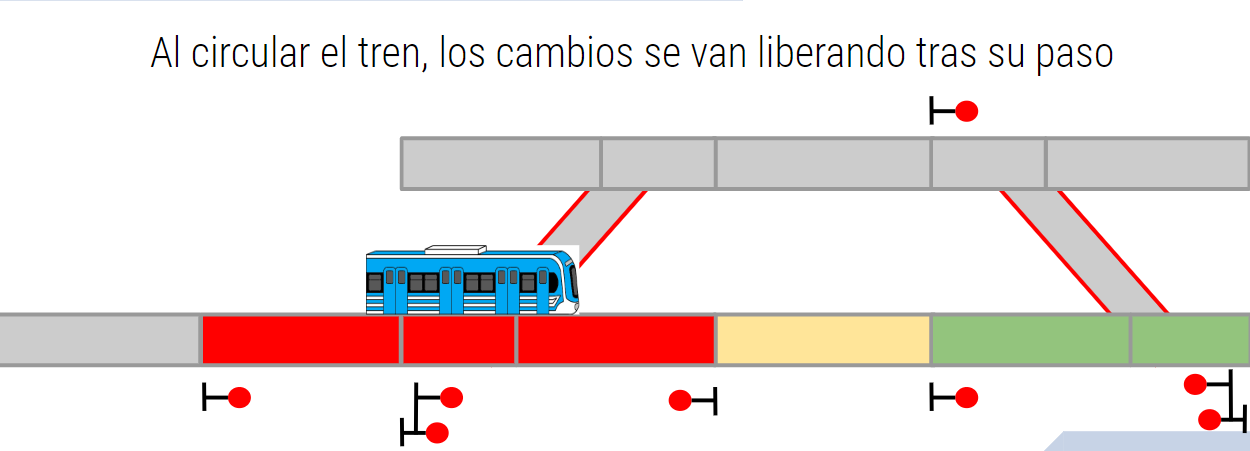
\includegraphics[width=1\textwidth]{Figuras/secuencial_2}
    	 \centering\caption{Formación activando el bloqueo por ocupación y el bloqueo por solape.}
    	 \label{fig:ACG_secuencial_2}
	\end{figure}
 
 	Una vez que la formación desocupa las secciones de vías asociadas al cambio de vías anterior, el sistema de enclavamientos libera inmediatamente toda la infraestructura asociada, como se ilustra en la Figura \ref{fig:ACG_secuencial_3}. A la vez, el sistema de enclavamientos debe esperar a que se cumpla el plazo de seguridad antes de liberar la infraestructura posterior al fin de la ruta. Solamente son liberadas las secciones y señales que ya no son conflictivas.
	   
	\begin{figure}[!h]
	  \centering
	  
\includegraphics[width=1\textwidth]{Figuras/secuencial_3}
	  \centering\caption{Liberación secuencial de la infraestructura por detrás de la formación.}
	  \label{fig:ACG_secuencial_3}
	\end{figure}
 
 	Transcurrido el tiempo de seguridad, el sistema de enclavamientos libera las secciones, cambios de vías, señales y toda infraestructura posterior al fin de la ruta, tal como se ilustra en la Figura \ref{fig:ACG_secuencial_4}.

	 \begin{figure}[!h]
	     \centering
	     
\includegraphics[width=1\textwidth]{Figuras/secuencial_4}
	     \centering\caption{Liberación secuencial de la infraestructura por delante de la formación.}
	     \label{fig:ACG_secuencial_4}
	 \end{figure}
	    
	El ACG implementa estas funcionalidades de seguridad para cada sistema de enclavamientos generado. 
	
	En las siguientes secciones se profundizará en la implementación de cada uno de los módulos del sistema y su comportamiento dinámico.